The simulation starts off with a normal image containing a 360\textdegree{}
panorama. The field of view of the camera is computed given its orientation
(normal Euler angles) and the actual camera image is created by sampling the
panorama image (the ground truth map) using raycasting. The camera is then
rotated by a tiny amount to get a second image patch. These patches are then
subtracted to get a list of events where the difference exceeds a threshold. To
also detect changes with a small absolute gradient, differences are accumulated
over time as it would happen with the real DVS. See figure \ref{fig:simulation}
for an example output.

This discrete approach is fairly straightforward but suffers from the problem
that it is very slow, as extremely tiny steps have to be taken to get accurate
events.

\begin{figure}
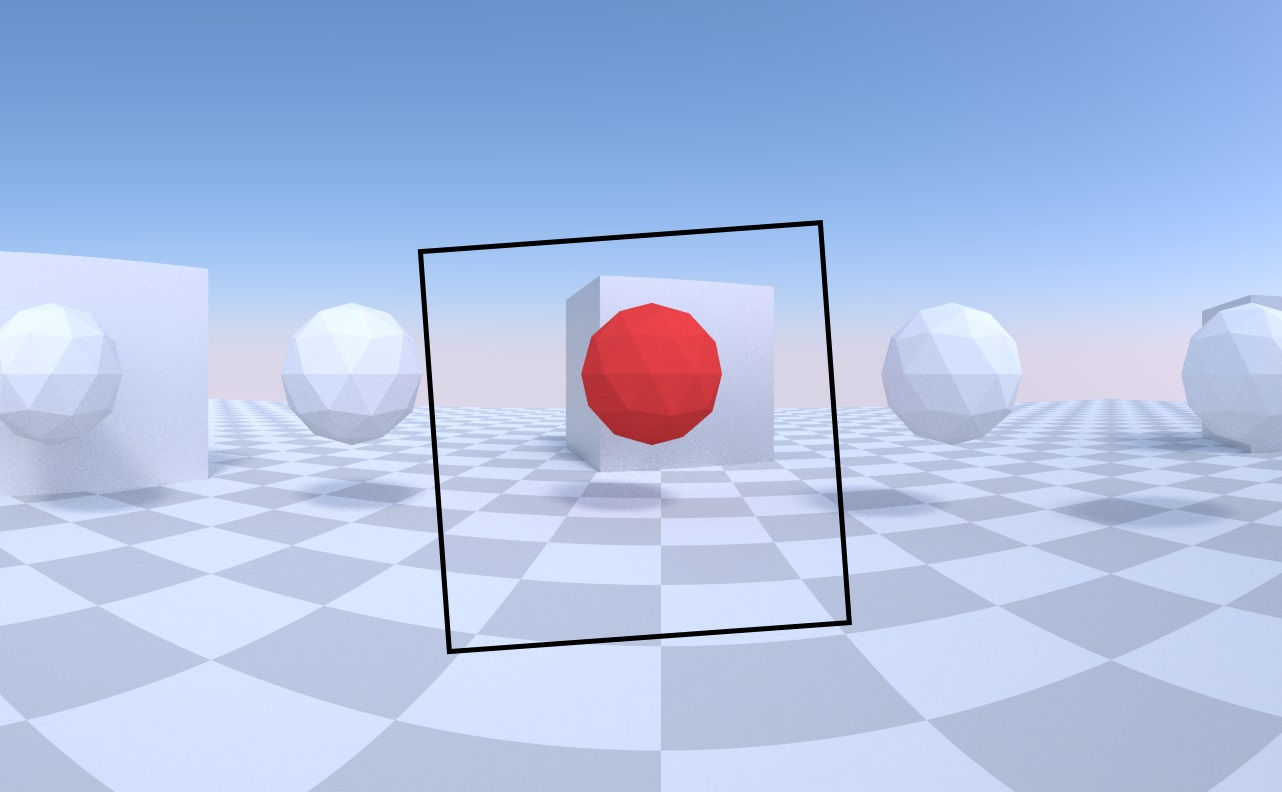
\includegraphics[width=\linewidth]{images/simulation_raw.jpg}
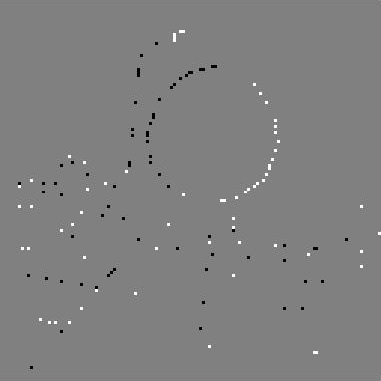
\includegraphics[width=\linewidth]{images/simulation_events.jpg}
\caption{above: the map used as input with the camera's FOV, below: events generated by moving the camera to the right}
\label{fig:simulation}
\end{figure}
